\documentclass[oneside, final, 14pt]{extarticle}
\usepackage[T2A]{fontenc}
\usepackage[utf8x]{inputenc}
\usepackage[english,russian]{babel}
\usepackage{listings}
\usepackage{xcolor}
\usepackage{lmodern}
\usepackage{textcomp}
\usepackage{lastpage}
\usepackage{vmargin}
\usepackage{titlesec}
\usepackage{mathptmx}
\usepackage{amsmath}
\usepackage{amssymb}
\usepackage{amsthm}
\usepackage{graphicx}
\usepackage{subfig}
\usepackage{pgf}
\usepackage{float}

\graphicspath{ {./screens/} }

\titlespacing*{\section}
{0pt}{5.5ex plus 1ex minus .2ex}{4.3ex plus .2ex}
\titlespacing*{\subsection}
{0pt}{5.5ex plus 1ex minus .2ex}{4.3ex plus .2ex}
\setpapersize{A4}
\setmarginsrb{2cm}{1.5cm}{1.5cm}{1.5cm}{0pt}{0mm}{0pt}{13mm}
\sloppy
\linespread{1.3}


\definecolor{mGreen}{rgb}{0,0.6,0}
\definecolor{mGray}{rgb}{0.5,0.5,0.5}
\definecolor{mPurple}{rgb}{0.58,0,0.82}
\definecolor{maroon}{rgb}{0.5,0,0}
\definecolor{darkgreen}{rgb}{0,0.5,0}

\lstdefinelanguage{XML}
{
  basicstyle=\ttfamily,
  morestring=[s]{"}{"},
  morecomment=[s]{?}{?},
  morecomment=[s]{!--}{--},
  commentstyle=\color{darkgreen},
  moredelim=[s][\color{black}]{>}{<},
  moredelim=[s][\color{red}]{\ }{=},
  stringstyle=\color{blue},
  identifierstyle=\color{maroon}
}

\lstdefinestyle{CStyle}{,   
    commentstyle=\color{mGreen},
    keywordstyle=\color{magenta},
    stringstyle=\color{mPurple},
    basicstyle=\footnotesize,
    breakatwhitespace=false,         
    breaklines=true,                 
    captionpos=b,                    
    keepspaces=true,                 
    showspaces=false,                
    showstringspaces=false,
    showtabs=false,                  
    tabsize=2,
    language=C
}

\begin{document}

\normalsize

\begin{titlepage}
\begin{center}
\textsc{Московский Государственный Университет имени М.В. Ломоносова\\[5mm]
Факультет вычислительной математики и кибернетики}
\centerline{\hfill\hrulefill\hrulefill\hfill}
\end{center}

\vfill
\vfill
\vfill
\vfill
\begin{center}
\Large
\textbf{Отчёт по теоретическому заданию в рамках курса \\
«Суперкомпьютерное моделирование и технологии»}
\end{center}

\vfill
\vfill
\vfill
\hfill
\begin{flushright}
Вариант 181
\end{flushright}
    
\begin{flushright}
Выполнил: \\
Шорошов Григорий Максимович, \\
622 группа \\[5mm]
\end{flushright}

\vfill
\vfill
\vfill
\begin{center}
Москва, \the\year
\end{center}
\end{titlepage}
 
\parindent=1cm

\newpage
\section*{Исходный фрагмент и описание информационной \\ структуры}
В качестве условия задачи выступает фрагмент программы на языке C, листинг которой приведён
в Приложении 1. Требовалось выполнить исследование информационной структуры этого
фрагмента, то есть выявить имеющиеся в ней зависимости по данным и их характер, после чего
составить описание информационной структуры на языке разметки Algolang. Итоговый листинг
описания структуры фрагмента на языке Algolang получился вот таким:

\lstset{language=XML}
\begin{minipage}{0.9\linewidth}
\begin{lstlisting}[
    basicstyle=\footnotesize, showstringspaces=false
]
<?xml version="1.0" encoding="UTF-8"?>
<algo>
    <params>
        <param name="N" type="int" value="5"></param>
        <param name="M" type="int" value="4"></param>
    </params>
    <block id="0" dims="1">
        <arg name="i" val="2..N+1"></arg>
        <vertex condition="" type="1">
        </vertex>
    </block>
    <block id="1" dims="2">
        <arg name="i" val="2..N+1"></arg>
        <arg name="j" val="2..M+1"></arg>
        <vertex condition="" type="2">
            <in src="i - 1, j"></in>
            <in bsrc="0" src="i"></in>
        </vertex>
    </block>
    <block id="2" dims="3">
        <arg name="i" val="2..N+1"></arg>
        <arg name="j" val="1..M+1"></arg>
        <arg name="k" val="1..N"></arg>
        <vertex condition="(j == 1) and (k == 1)" type="3">
            <in bsrc="0" src="N + 1"></in>
        </vertex>
        <vertex condition="(j > 1)" type="3">
            <in src="i, j - 1, k - 1"></in>
        </vertex>
    </block>
</algo>
\end{lstlisting}
\end{minipage}

\section*{Информационный граф фрагмента и его свойства}

В соответствии с инструкциями к системе Algoload я зашёл в неё под своим логином
ucmc2020ss181 и загрузил в систему описание информационной структуры из предыдущего
пункта. В окне просмотра оказалась следующая визуализация информационного графа:

\newlength{\mygraphwidth}\setlength{\mygraphwidth}{0.9\textwidth}

\begin{figure}[H]
    \centering
    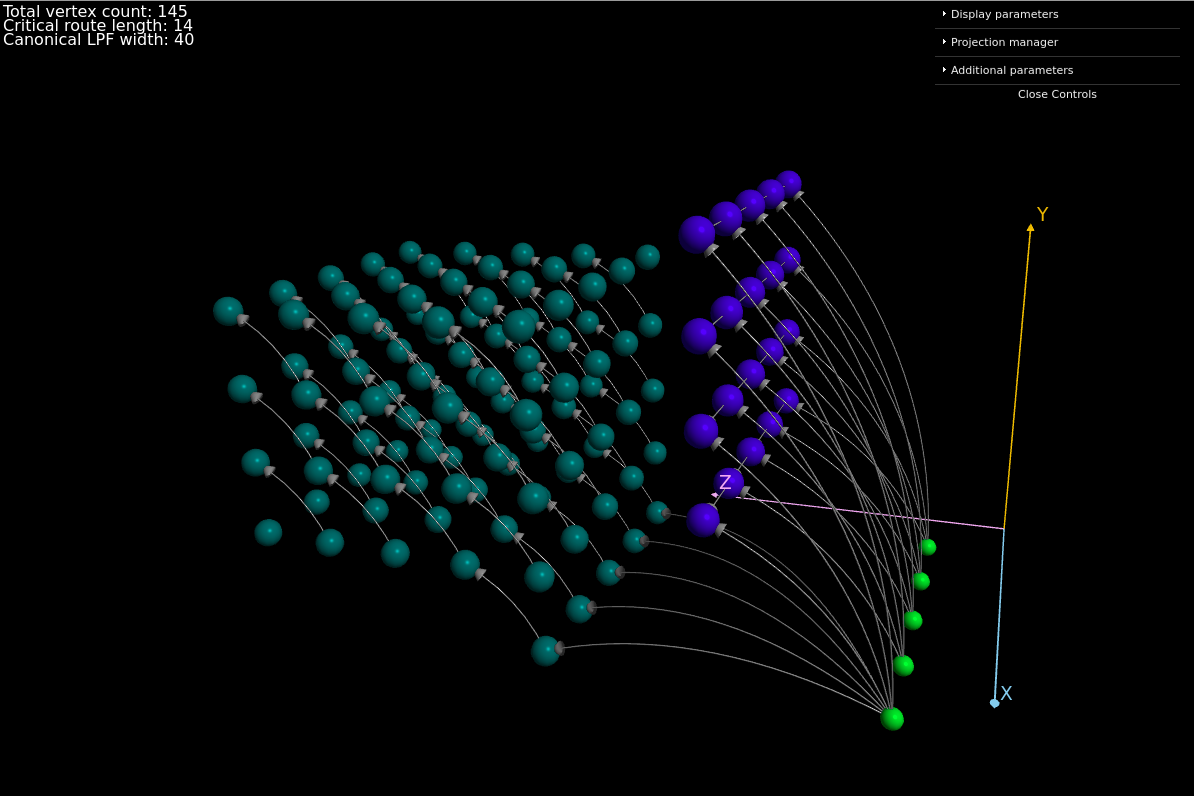
\includegraphics[width=\mygraphwidth]{1.png}
    \caption{Визуализация информационного графа}
\end{figure}

\begin{figure}[H]
    \centering
    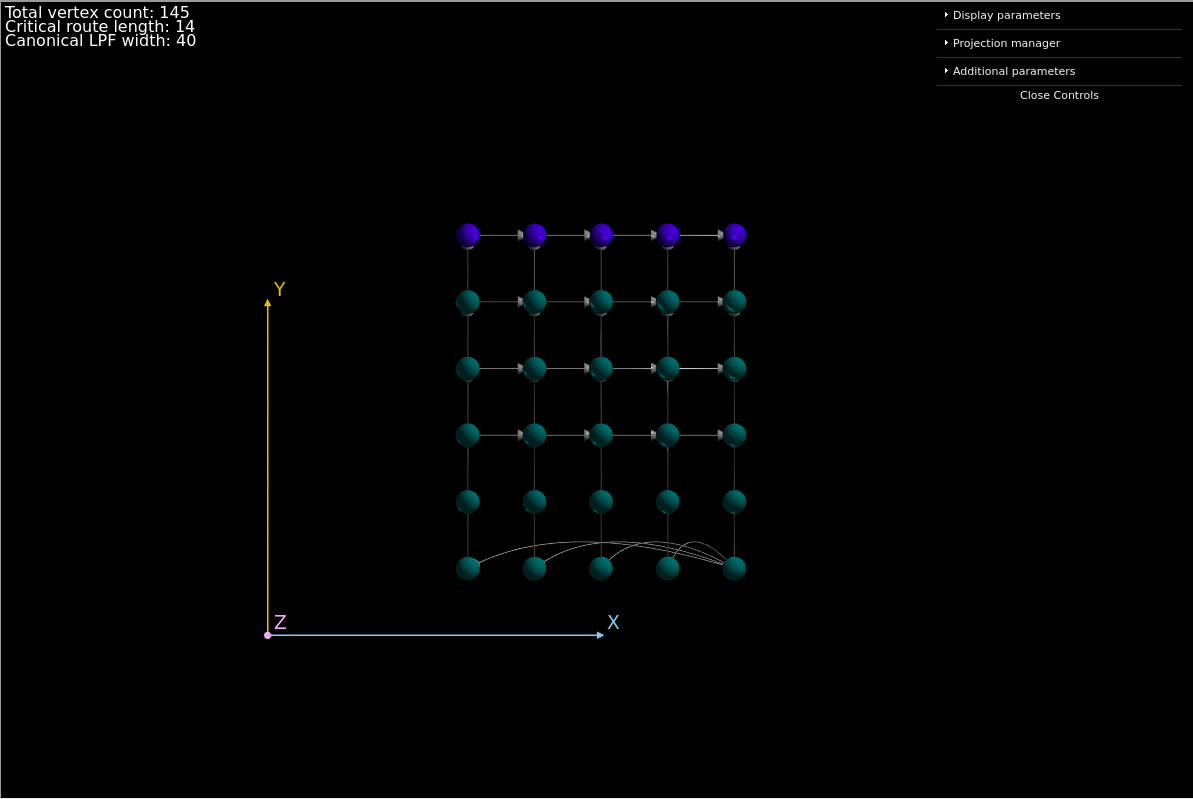
\includegraphics[width=\mygraphwidth]{2.png}
    \caption{Проекция oXY}
\end{figure}

\begin{figure}[H]
    \centering
    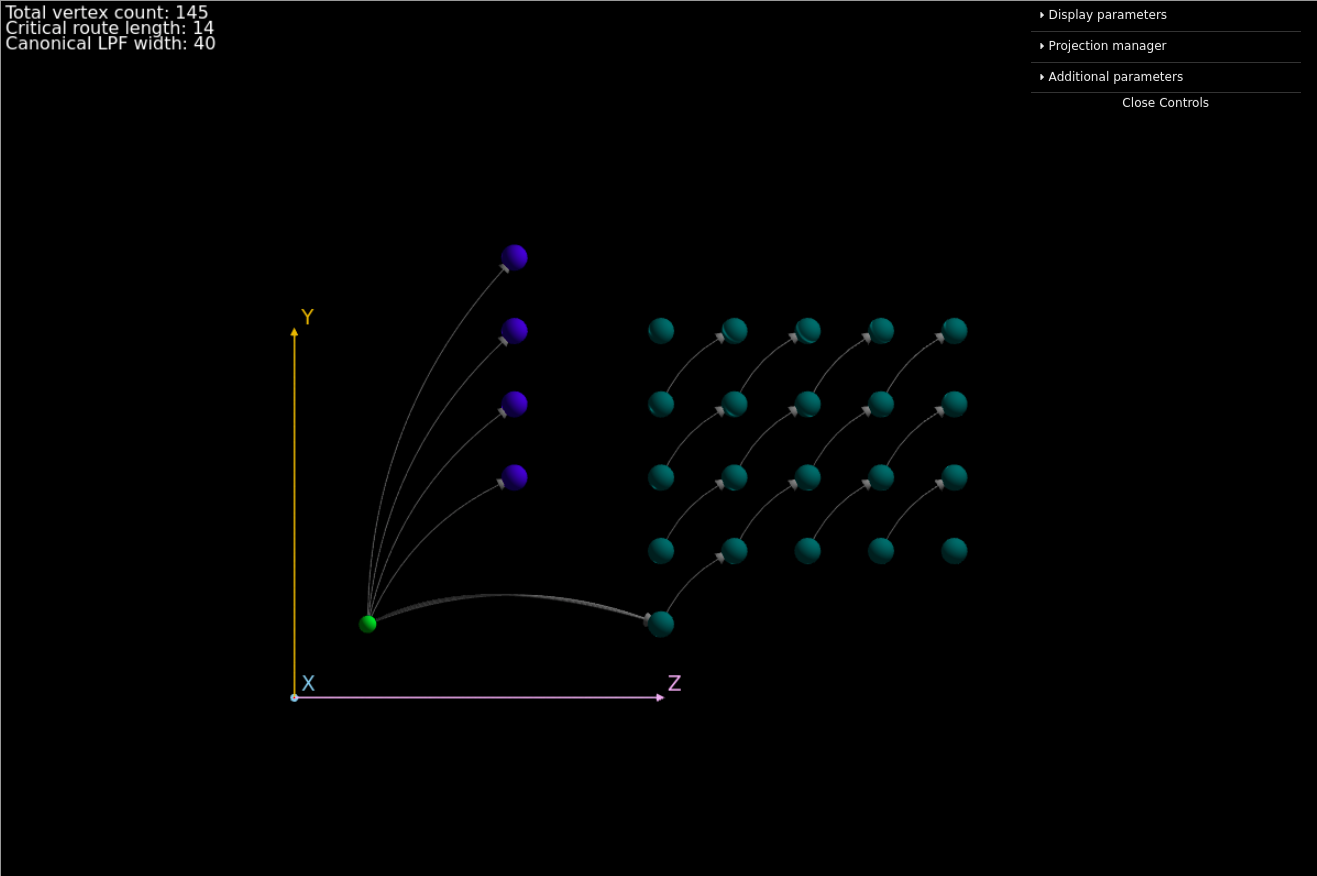
\includegraphics[width=\mygraphwidth]{3.png}
    \caption{Проекция oYZ}
\end{figure}

\begin{figure}[H]
    \centering
    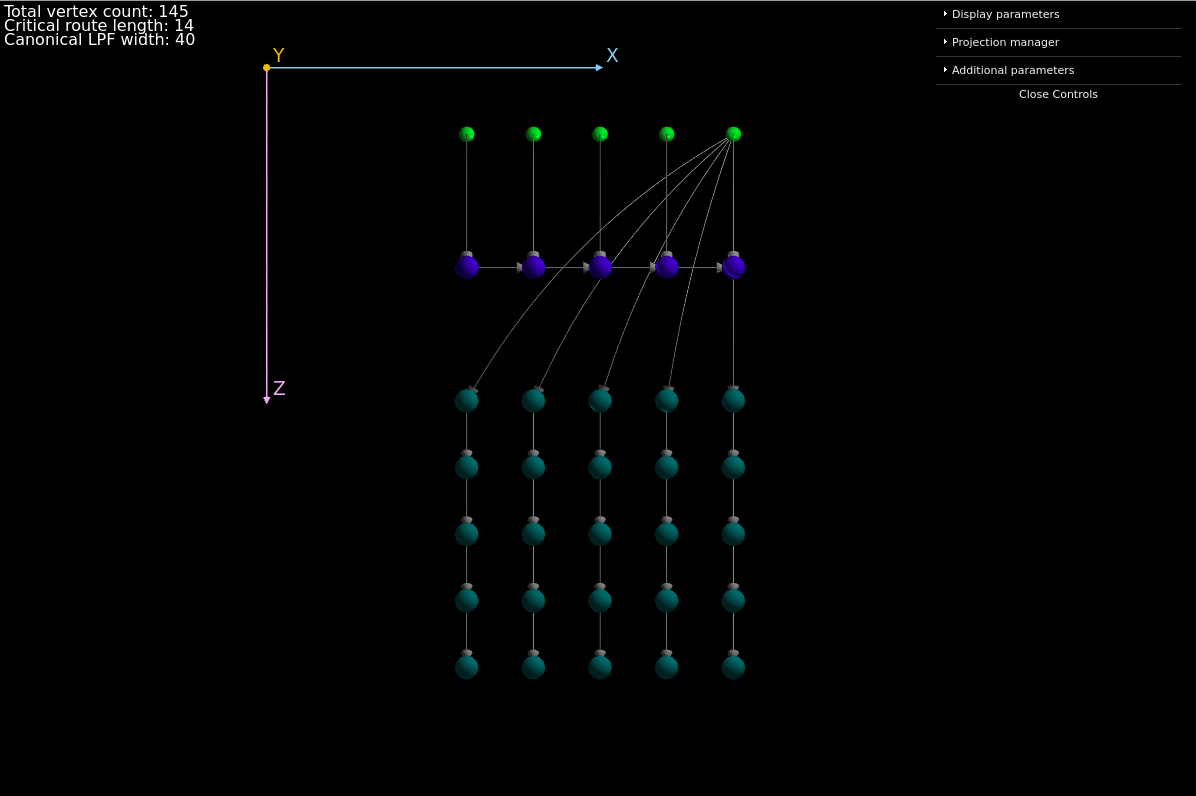
\includegraphics[width=\mygraphwidth]{4.png}
    \caption{Проекция oXZ}
\end{figure}

Базовые свойства информационного графа оказались следующими:

\begin{enumerate}
    \item Число вершин и информационном графе для заданных значений внешних параметров --- 130.
    Число вершин $ C $ для произвольного значения $ M  $ и $ N $ выражается формулой $ C = 2N + N(N + 1)M $.
    \item Длина критического пути в графе для заданных значений параметров --- 5. В общем случае она равна $ N $.
    \item Ширина канонической ЯПФ W оказалась равной 40. В общем случае она задаётся
    формулой
    $$
    W =
    \begin{cases}
      M + N(M + N - 3)       & \quad \text{если } M > 2N\\
      N(N + M - 1)  & \quad \text{иначе}
    \end{cases}
    $$
    \item Максимальная глубина вложенности циклов равна 3.
    \item В данном информационном графе присутствует 11 различных типов дуг. В общем случае число различных типов дуг $ E $ выражается
    формулой $ E =  M + N + 2 $.
    \item Длинные дуги присутствуют, их число равно 5, а в общем случае – $ N $.
\end{enumerate}

\section*{Приложение 1}

Листинг исходного фрагмента на C

\begin{minipage}{0.9\linewidth}
\begin{lstlisting}[language=C, style=CStyle]
for (i = 2; i <= n + 1; ++i)
    C[i] = C[i + 1] + D[i];
for (i = 2; i <= n + 1; ++i)
    for (j = 2; j <= m + 1; ++j)
        B[i][j] = B[i - 1][j] + C[i];
for (i = 2; i <= n + 1; ++i)
{
    A[i][1][1] = C[n + 1];
    for (j = 2; j <= m + 1; ++j)
        for (k = 1; k <= n; ++k)
            A[i][j][k] = A[i][j - 1][k - 1] + A[i][j][k];
}
\end{lstlisting}
\end{minipage}

\section*{Приложение 2}

Фрагмент с разметкой параллельных циклов с использованием директивы OpenMP \emph{\#pragma omp parallel for}:

\begin{minipage}{0.9\linewidth}
\begin{lstlisting}[language=C, style=CStyle]
for (i = 2; i <= n + 1; ++i)
    C[i] = C[i + 1] + D[i];
for (i = 2; i <= n + 1; ++i)
    #pragma omp parallel for
    for (j = 2; j <= m + 1; ++j)
        B[i][j] = B[i - 1][j] + C[i];
#pragma omp parallel for
for (i = 2; i <= n + 1; ++i)
{
    A[i][1][1] = C[n + 1];
    for (j = 2; j <= m + 1; ++j)
        #pragma omp parallel for
        for (k = 1; k <= n; ++k)
            A[i][j][k] = A[i][j - 1][k - 1] + A[i][j][k];
}
\end{lstlisting}
\end{minipage}

\end{document}